\documentclass{beamer}

\usepackage[utf8]{inputenc}
\usepackage{default}

\usetheme{CambridgeUS}
%\usecolortheme{seagull}
%\useoutertheme{tree}
\beamertemplatenavigationsymbolsempty
\hypersetup{pdfstartview={Fit}}
\title[Behavior Based Architectures]{Behavior Based Systems}
\author{Luke Fraser}
\date{\today}
\begin{document}

\begin{frame}
 \titlepage
\end{frame}

\begin{frame}{Overview}
 \begin{itemize}
  \item Robot Control Architectures
  \item Behavior Based Systems
  \item Representation
  \item Learning
 \end{itemize}
\end{frame}
\section{Robot Control Architectures}
\begin{frame}{Robot Control Architectures}
 \begin{itemize}
  \item Deliberative - Think, Then Act
  \item Reactive - Don't Think, Act
  \item Hybrid - Think and Act Concurrently
  \item Behavior Based - Think the Way You Act
 \end{itemize}
\end{frame}

\begin{frame}{Deliberative - Think, Then Act}
 \begin{itemize}
  \item Planning
  \item SPA - Sense Plan Act
  \item Pros
  \begin{itemize}
   \item Optimal Solution - \emph{If computationally feasible.}
   \item A good solution in a world that does not change.
  \end{itemize}
  \item Cons
  \begin{itemize}
   \item Slow
   \item Dynamic environments
   \begin{itemize}
    \item Environment will change during deliberation stage.
    \item Solution only correct for previous time-slice.
   \end{itemize}
  \end{itemize}
 \end{itemize}
\end{frame}

\begin{frame}{Reactive - Don't Think, Act}
 \begin{columns}[T]
  \begin{column}[T]{6cm}
  \begin{itemize}
    \item No Planning
    \item No world model
    \item Pros
    \begin{itemize}
    \item Fast
    \item Perform simple tasks well
    \item Emergent behavior
    \end{itemize}
    \item Cons
    \begin{itemize}
    \item No Planning
    \item Limited functionality
    \item Emergent behavior
    \end{itemize}
  \end{itemize}
  \end{column}
  \begin{column}[T]{4cm}
  \centering
   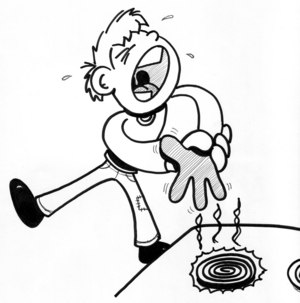
\includegraphics[width=4cm]{stove.jpg}
  \end{column}
 \end{columns}
\end{frame}

\begin{frame}{Hybrid - Think and Act Concurrently}
 \begin{itemize}
  \item Deliberative \& Reactive
  \item Pros
  \begin{itemize}
   \item Fast reaction times
   \item Can perform complex actions.
  \end{itemize}
  \item Cons
  \begin{itemize}
   \item Deliberative and reactive layers interfere.
   \item Intermediat layer is difficult to develop. - Which layer is right?
  \end{itemize}
 \end{itemize}
\end{frame}

\begin{frame}{Behavior Based - Think the Way You Act}
 
\end{frame}

\section{Behavior Based Systems}
\begin{frame}{Behavior Based Systems}
 \begin{itemize}
  \item Misconceptions
 \end{itemize}

\end{frame}

\section{Representation}
\section{Learning}
\end{document}
